\section{Thực nghiệm và phân tích kết quả}
\subsection{Các chỉ số chính để đánh giá hiệu quả của bài toán 2DCSP}

\hspace{0.5cm}Để đánh giá hiệu quả của các thuật toán giải 2DCSP, chúng ta xem xét các chỉ số chính sau:

\begin{itemize}
    \item \textbf{Mức độ lãng phí vật liệu:} Đánh giá tỷ lệ phần trăm diện tích vật liệu đầu vào được sử dụng hiệu quả. Chỉ số này được tính bằng công thức:
    \[
    \text{Mức độ lãng phí vật liệu} = \frac{\text{Tổng diện tích các mảnh cắt}}{\text{Tổng diện tích vật liệu đã sử dụng}} \times 100\%.
    \]
    Giá trị càng thấp thể hiện khả năng sử dụng vật liệu càng hiệu quả.
    
    Giá trị vật liệu càng thấp chứng tỏ mẫu cắt được tối ưu hơn.

    \item \textbf{Thời gian tính toán:} Thời gian mà thuật toán cần để tìm ra lời giải, đặc biệt quan trọng khi đánh giá khả năng mở rộng đối với các tập dữ liệu lớn.

    \item \textbf{Đáp ứng nhu cầu sản phẩm:} Đánh giá mức độ đáp ứng nhu cầu sản xuất bằng cách kiểm tra số lượng sản phẩm đã thực hiện cắt.

    \item \textbf{Giảm thiểu số lượng tấm vật liệu:} So sánh tổng số tấm vật liệu được sử dụng với số lượng tối thiểu lý thuyết cần thiết.
\end{itemize}

\subsubsection{Tóm tắt các chỉ số chính}

Bảng dưới đây tóm tắt các chỉ số chính để đánh giá hiệu quả của các thuật toán:

\begin{table}[H]
    \centering
    \renewcommand{\arraystretch}{1.5}
    \begin{tabular}{|l|p{1.5cm}|p{6cm}|p{1.3cm}|}
     \hline
        \textbf{Chỉ số}               & \textbf{Đơn vị}                 & \textbf{Mô tả}                                                                                 & \textbf{Mức độ quan trọng}  \\ \hline
        Mức độ lãng phí vật liệu    & \%                            & tỷ lệ phần trăm diện tích vật liệu đầu vào được sử dụng
hiệu quả.                                          & Cao \\ \hline
        Thời gian tính toán           & giây                          & Thời gian cần để tính toán lời giải.                                                            & Vừa                   \\ \hline
        Đáp ứng nhu cầu               & sản phẩm                            & Số lượng nhu cầu sản phẩm được đáp ứng.                                                            & Vừa  \\ \hline
        Số lượng tấm vật liệu         & \text{tấm}                    & Tổng số tấm vật liệu sử dụng so với số lượng tối thiểu lý thuyết.                               & Cao                   \\ \hline
    \end{tabular}
    \caption{Các chỉ số chính để đánh giá hiệu quả của bài toán 2DCSP}
    \label{tab:key_metrics}
\end{table}

\subsection{Đánh giá kết quả thực nghiệm}
\subsubsection{Môi trường thực nghiệm}

Các thử nghiệm được thực hiện trên một hệ thống có cấu hình như sau:

\begin{itemize}
    \item \textbf{Hệ điều hành (OS):} Windows 10 Pro, phiên bản Build 22H2 (19045).
    \item \textbf{Độ phân giải màn hình:} 1920x1080 @60Hz.
    \item \textbf{Bộ xử lý (CPU):} Intel(R) Core(TM) i7-8550U CPU @ 1.80GHz.
    \item \textbf{Đồ họa (GPU):} Intel(R) UHD Graphics 620.
    \item \textbf{Bộ nhớ (RAM):} 8493 MB / 16278 MB (52\% đang sử dụng).
    \item \textbf{Dung lượng đĩa (Disk):} Ổ đĩa C:\ có tổng dung lượng 104.84 GB (còn trống 11.07 GB).
\end{itemize}

Chúng tôi sử dụng ngôn ngữ lập trình Python để mô phỏng và kiểm thử hai thuật toán nói trên trên cùng tập dữ liệu. Tập dữ liệu được sử dụng có thể truy cập tại liên kết sau: \href{https://raw.githubusercontent.com/nhan2892005/ReinforcementLearning/refs/heads/main/CSP/results.csv}{Dữ liệu kiếm thử}.

Biểu đồ dưới đây minh họa phân bố dữ liệu trong quá trình kiểm thử:

\begin{figure}[H]
    \centering
    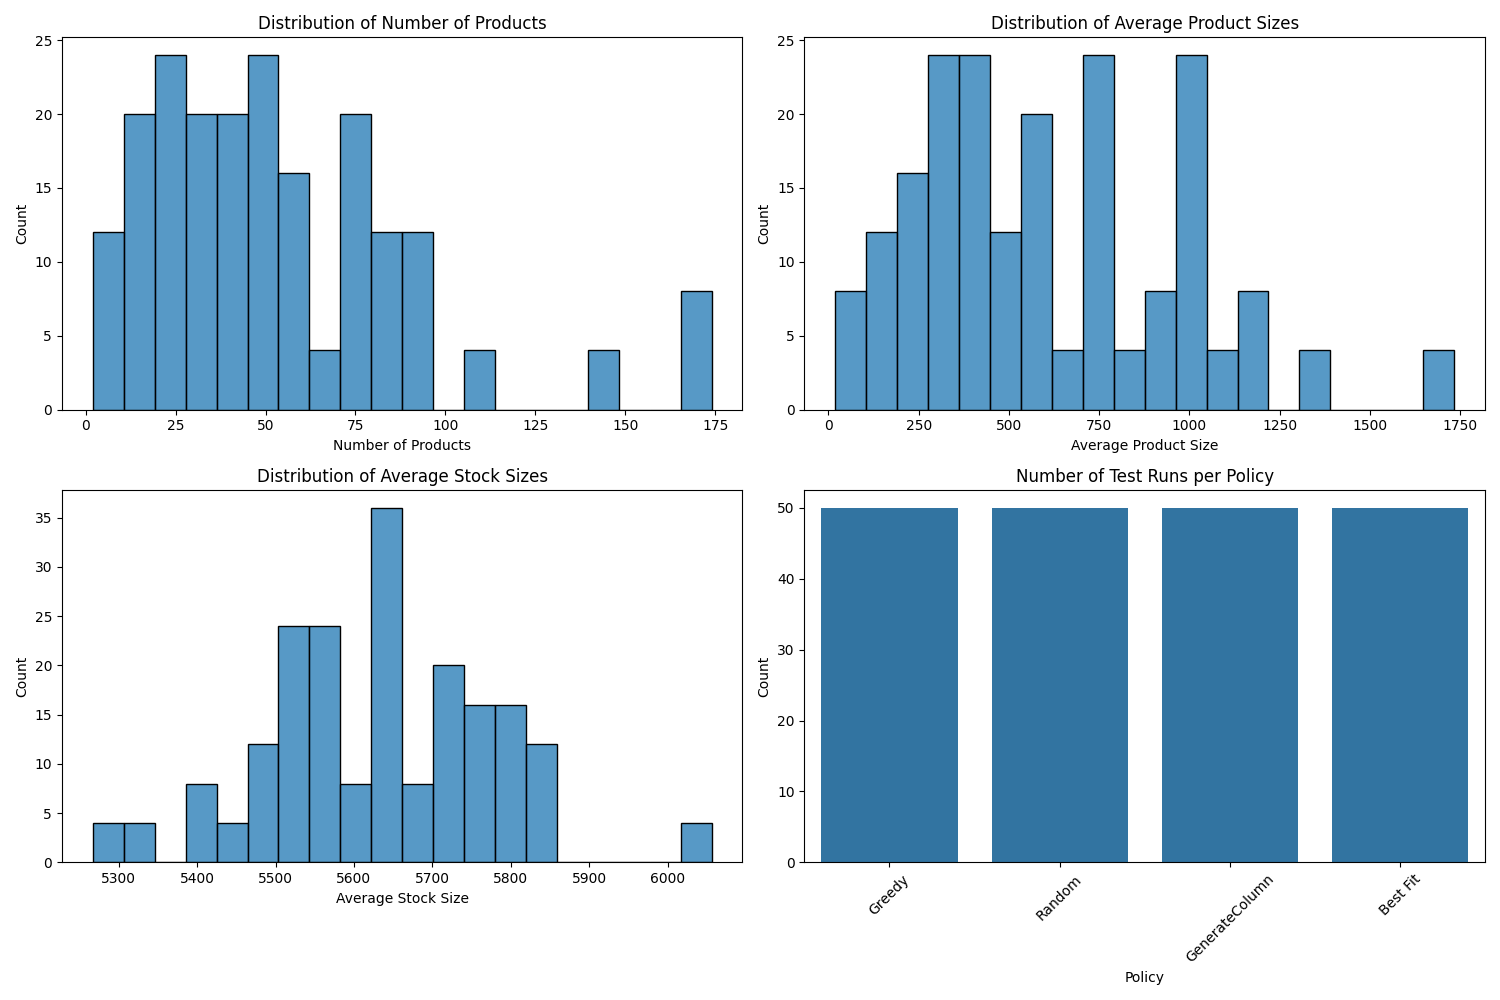
\includegraphics[width=0.8\textwidth]{Images/test_case_distributions.png}
    \caption{Phân bố số lượng sản phẩm, kích thước sản phẩm trung bình, kích thước kho trung bình, và số lần chạy thử nghiệm cho mỗi chính sách.}
    \label{fig:test_distributions}
\end{figure}

\textbf{Mô tả biểu đồ:}
\begin{itemize}
    \item \textbf{Phân bố số lượng sản phẩm:} Biểu đồ trên bên trái cho thấy số lượng sản phẩm được phân bố từ khoảng 0 đến 175 sản phẩm, với phần lớn rơi vào khoảng 25-75 sản phẩm.
    \item \textbf{Phân bố kích thước sản phẩm trung bình:} Biểu đồ trên bên phải minh họa các kích thước trung bình của sản phẩm, tập trung nhiều trong khoảng 250-1000 đơn vị.
    \item \textbf{Phân bố kích thước kho trung bình:} Biểu đồ dưới bên trái cho thấy kích thước kho trung bình dao động từ 5300 đến 6000 đơn vị, với phần lớn các trường hợp tập trung gần 5600 đơn vị.
    \item \textbf{Số lần chạy thử nghiệm:} Biểu đồ dưới bên phải thể hiện số lần thử nghiệm thực hiện cho từng chính sách. Tất cả các chính sách (Greedy, Random, GenerateColumn, và Best Fit) đều có số lần chạy thử nghiệm bằng nhau là 50 lần, và mỗi lần đều chạy trên cùng 1 bộ dữ liệu kiểm thử.
\end{itemize}

\subsubsection{Phân tích kết quả thí nghiệm}

Kết quả thí nghiệm được thể hiện qua bốn biểu đồ, bao gồm: \textit{Waste Percentage by Policy}, \textit{Number of Used Stocks by Policy}, \textit{Execution Time by Policy}, và \textit{Waste vs Number of Products}. Dưới đây là các phân tích chi tiết:


\begin{table}[!htp]
    \centering
    \begin{tabular}{|c|c|c|c|} \hline 
       \textbf{  Policy}&  \textbf{Avg Stock Use}d&  \textbf{Trim Loss} (\%)& \textbf{ Avg Runtime (s)}
\\ \hline 
         Best Fit&  5.4&  2.36&  2.106
\\ \hline 
         Generate Column&  5.08&  1.92&  10.560
\\ \hline 
         Greedy&  9.74&  3.08&  7.824
\\ \hline 
         Random&  41.14&  35.31&  0.009\\ \hline
    \end{tabular}
    \caption{Bảng số liệu giá trị trung bình các chỉ số của các thuật toán}
    \label{tab:result}
\end{table}

\begin{itemize}
    \item \textbf{Phần trăm lãng phí theo chính sách (Waste Percentage by Policy):} 
    \begin{itemize}
        \item Chính sách \textit{Greedy}, \textit{GenerateColumn}, và \textit{Best Fit} đều có phần trăm lãng phí thấp, với đa số giá trị tập trung gần mức 0-10\%. Điều này cho thấy ba chính sách này hiệu quả hơn trong việc giảm lãng phí.
        \item Ngược lại, chính sách \textit{Random} có sự biến thiên lớn và lãng phí cao hơn đáng kể, với mức trung bình dao động quanh 40\%. Đây là lựa chọn kém hiệu quả nhất.
    \end{itemize}

    \begin{figure}[!htp]
        \centering
        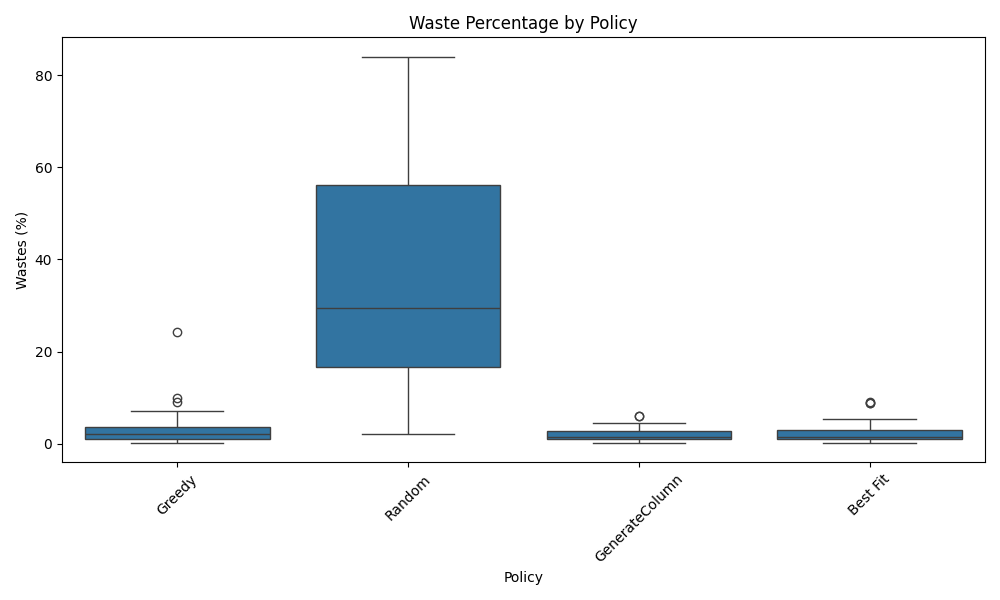
\includegraphics[width=0.5\linewidth]{Images/waste_comparison.png}
        \caption{Biểu đồ hộp thể hiện mức độ lãng phí trung bình của các chính sách}
        \label{fig:trimloss}
    \end{figure}
    
    \item \textbf{Số lượng vật liệu sử dụng theo chính sách (Number of Used Stocks by Policy):}
    \begin{itemize}
        \item Chính sách \textit{Greedy}, \textit{GenerateColumn}, và \textit{Best Fit} tiếp tục thể hiện sự ổn định, với số lượng kho sử dụng thấp và ít biến thiên.
        \item Chính sách \textit{Random} có số lượng vật liệu sử dụng lớn nhất và phân bố rộng, cho thấy sự có thể gây nhiều lãng phí trong việc tận dụng không gian lưu trữ.
    \end{itemize}
    \begin{figure}[!htp]
        \centering
        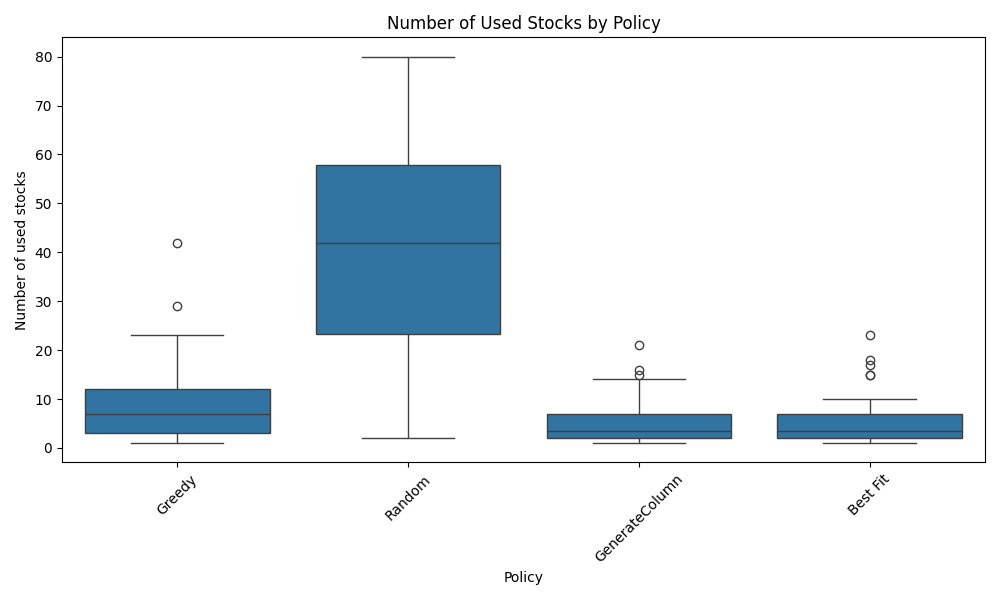
\includegraphics[width=0.5\linewidth]{Images/stocks_comparison.png}
        \caption{Biểu đồ hộp thể hiện số lượng vật liệu trung bình các chính sách sử dụng}
        \label{fig:stocks}
    \end{figure}
    
    \item \textbf{Thời gian thực thi theo chính sách (Execution Time by Policy):}
    \begin{itemize}
        \item Chính sách \textit{Greedy} và \textit{Best Fit} có thời gian thực thi thấp nhất, hầu hết dưới 5 giây. Điều này cho thấy chúng vừa hiệu quả về mặt chi phí lưu trữ, vừa nhanh về thời gian xử lý.
        \item Chính sách \textit{Generate Column} có thời gian thực thi cao hơn, với một số trường hợp cao gấp 5 lần trở lên so với các thuật toán khác. Mặc dù hiệu quả giảm lãng phí tốt, thời gian thực thi là một nhược điểm cần lưu ý.
    \end{itemize}
    \begin{figure}[!htp]
        \centering
        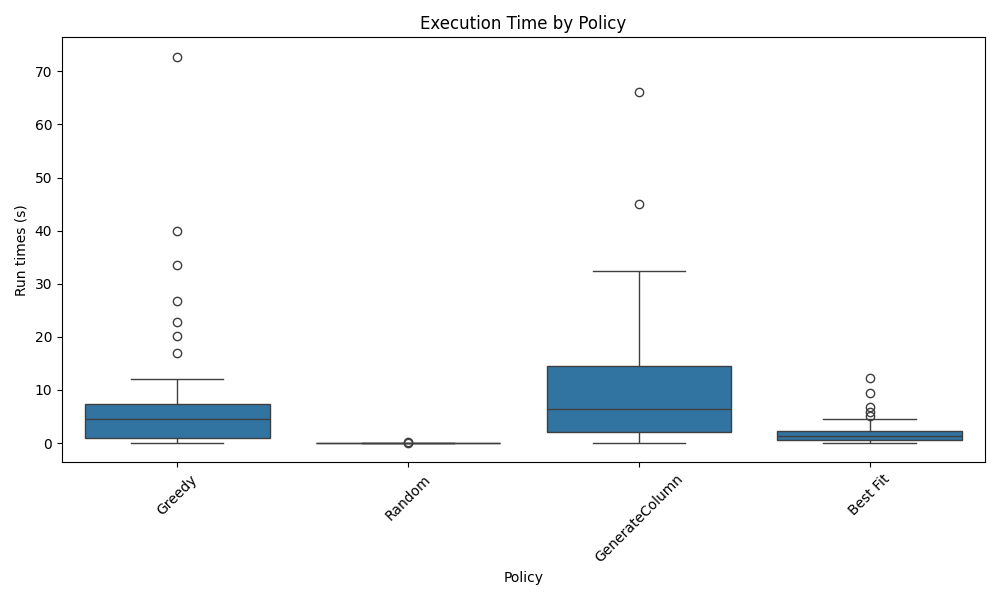
\includegraphics[width=0.5\linewidth]{Images/execution_time_comparison.png}
        \caption{Biểu đồ hộp thể hiện thời gian xử lý trung bình các chính sách sử dụng}
        \label{fig:time}
    \end{figure}
    
    \item \textbf{Lãng phí so với số lượng sản phẩm (Waste vs Number of Products):}
    \begin{itemize}
        \item Biểu đồ phân tán cho thấy chính sách \textit{Random} tạo ra sự gia tăng đáng kể về phần trăm lãng phí khi số lượng sản phẩm tăng, chứng minh đây là chính sách không phù hợp với các tập dữ liệu lớn.
        \item Các chính sách còn lại giữ được mức lãng phí thấp, gần như không bị ảnh hưởng bởi sự gia tăng số lượng sản phẩm. Điều này khẳng định khả năng thích nghi tốt của các chính sách \textit{Greedy}, \textit{GenerateColumn}, và \textit{Best Fit}.
    \end{itemize}
    \begin{figure}[!htp]
        \centering
        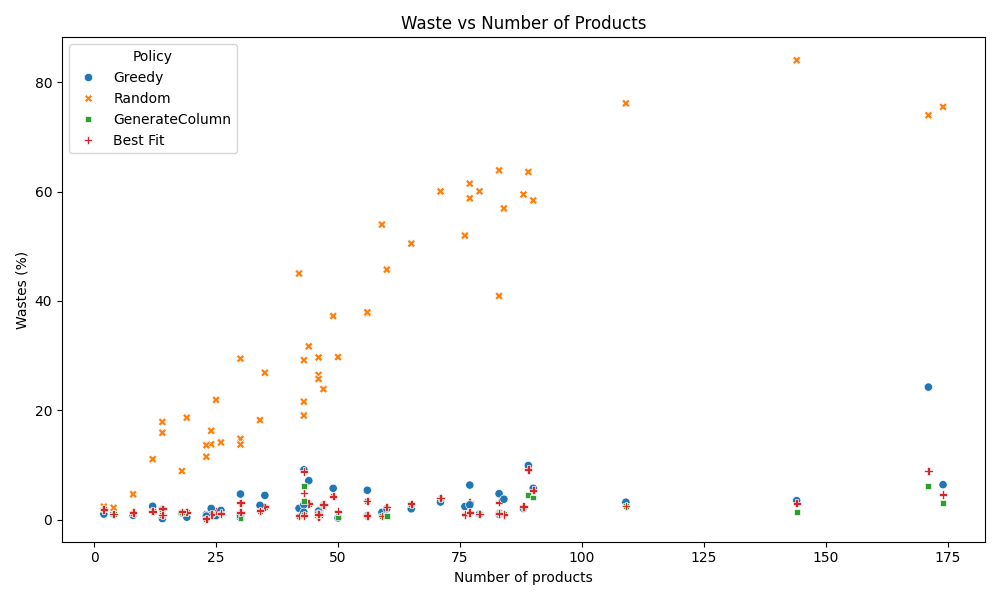
\includegraphics[width=0.5\linewidth]{Images/waste_vs_products.png}
        \caption{Biểu đồ phân tán thể hiện mối quan hệ giữa phần trăm lãng phí và số lượng sản phẩm}
        \label{fig:time}
    \end{figure}
\end{itemize}

\textbf{Kết luận:} Chính sách \textit{Greedy}, \textit{GenerateColumn}, và \textit{Best Fit} đều thể hiện sự tối ưu vượt trội về mặt giảm lãng phí và sử dụng kho lưu trữ. Trong đó, \textit{Best Fit} có ưu thế hơn về cả thời gian thực thi và tối thiểu mức độ lãng phí. Chính sách \textit{Random} tỏ ra không phù hợp cho các ứng dụng thực tế do lãng phí cao và hiệu suất thấp.


